%%%%%%%%%%%%%%%%%%%%%%%%%%%%%%%%%%%%%%%%%%%%%%%%%%%%%%%%%%%%%%%%%%%%%
%% This is a (brief) model paper using the achemso class
%% The document class accepts keyval options, which should include
%% the target journal and optionally the manuscript type.
%%%%%%%%%%%%%%%%%%%%%%%%%%%%%%%%%%%%%%%%%%%%%%%%%%%%%%%%%%%%%%%%%%%%%
\documentclass[journal=jctcce,manuscript=article]{achemso}
\setkeys{acs}{articletitle=false}

%%%%%%%%%%%%%%%%%%%%%%%%%%%%%%%%%%%%%%%%%%%%%%%%%%%%%%%%%%%%%%%%%%%%%
%% Place any additional packages needed here.  Only include packages
%% which are essential, to avoid problems later. Do NOT use any
%% packages which require e-TeX (for example etoolbox): the e-TeX
%% extensions are not currently available on the ACS conversion
%% servers.
%%%%%%%%%%%%%%%%%%%%%%%%%%%%%%%%%%%%%%%%%%%%%%%%%%%%%%%%%%%%%%%%%%%%%
\usepackage[version=3]{mhchem} % Formula subscripts using \ce{}
\usepackage{chemnum}
\usepackage{multirow}
\usepackage{textgreek}
\usepackage{textcomp}
\usepackage{setspace}
\usepackage{afterpage}
\usepackage{caption}
\usepackage{floatrow}
\usepackage{gensymb}

\usepackage[most]{tcolorbox}


\captionsetup{justification=raggedright,singlelinecheck=false}
\usepackage[labelfont=bf]{caption}
\usepackage{makecell}

\usepackage{dblfloatfix}
\usepackage{framed}

\usepackage{natbib}
\usepackage[acroymn]{glossaries}
\usepackage{tabularx} % for 'tabularx' environment
\usepackage{array}

\usepackage{acro}

\acsetup{hyperref=true}

\usepackage{enumitem}

\usepackage{multicol}
\usepackage{graphicx}
\usepackage{subcaption}

% glossary
\usepackage{hyperref}


\hypersetup{
    colorlinks,
    citecolor=black,
    filecolor=black,
    linkcolor=black,
    urlcolor=black
}



%%%%%%%%%%%%%%%%%%%%%%%%%%%%%%%%%%%%%%%%%%%%%%%%%%%%%%%%%%%%%%%%%%%%%
%% If issues arise when submitting your manuscript, you may want to
%% un-comment the next line.  This provides information on the
%% version of every file you have used.
%%%%%%%%%%%%%%%%%%%%%%%%%%%%%%%%%%%%%%%%%%%%%%%%%%%%%%%%%%%%%%%%%%%%%
%%\listfiles

%%%%%%%%%%%%%%%%%%%%%%%%%%%%%%%%%%%%%%%%%%%%%%%%%%%%%%%%%%%%%%%%%%%%%
%% Place any additional macros here.  Please use \newcommand* where
%% possible, and avoid layout-changing macros (which are not used
%% when typesetting).
%%%%%%%%%%%%%%%%%%%%%%%%%%%%%%%%%%%%%%%%%%%%%%%%%%%%%%%%%%%%%%%%%%%%%
\newcommand*\mycommand[1]{\texttt{\emph{#1}}}

%%%%%%%%%%%%%%%%%%%%%%%%%%%%%%%%%%%%%%%%%%%%%%%%%%%%%%%%%%%%%%%%%%%%%
%% Meta-data block
%% ---------------
%% Each author should be given as a separate \author command.
%%
%% Corresponding authors should have an e-mail given after the author
%% name as an \email command. Phone and fax numbers can be given
%% using \phone and \fax, respectively; this information is optional.
%%
%% The affiliation of authors is given after the authors; each
%% \affiliation command applies to all preceding authors not already
%% assigned an affiliation.
%%
%% The affiliation takes an option argument for the short name.  This
%% will typically be something like "University of Somewhere".
%%
%% The \altaffiliation macro should be used for new address, etc.
%% On the other hand, \alsoaffiliation is used on a per author basis
%% when authors are associated with multiple institutions.
%%%%%%%%%%%%%%%%%%%%%%%%%%%%%%%%%%%%%%%%%%%%%%%%%%%%%%%%%%%%%%%%%%%%%
\author{Eric D. Boittier}
\email{eric.boittier@uqconnect.edu.au}
\affiliation[UQ]{The University of Queendland, St Lucia, Queensland, Australia}

\author{\linebreak Supervisors: A/Professor Vito Ferro}
\affiliation[UQ]{The University of Queendland, St Lucia, Queensland, Australia}

\author{Dr Neha Gandhi}
\affiliation[QUT]{Queensland University of Technology, Gardens Point, Queensland, Australia}


%%%%%%%%%%%%%%%%%%%%%%%%%%%%%%%%%%%%%%%%%%%%%%%%%%%%%%%%%%%%%%%%%%%%%
%% The document title should be given as usual. Some journals require
%% a running title from the author: this should be supplied as an
%% optional argument to \title.
%%%%%%%%%%%%%%%%%%%%%%%%%%%%%%%%%%%%%%%%%%%%%%%%%%%%%%%%%%%%%%%%%%%%%
\title[Honours]
  {Parameterisation of ``VinaCarb" for improved docking of heparin/heparan sulfate  \linebreak \large Research Proposal}

%%%%%%%%%%%%%%%%%%%%%%%%%%%%%%%%%%%%%%%%%%%%%%%%%%%%%%%%%%%%%%%%%%%%%
%% Some journals require a list of abbreviations or keywords to be
%% supplied. These should be set up here, and will be printed after
%% the title and author information, if needed.
%%%%%%%%%%%%%%%%%%%%%%%%%%%%%%%%%%%%%%%%%%%%%%%%%%%%%%%%%%%%%%%%%%%%%
\abbreviations{IR,NMR,UV}
\keywords{American Chemical Society}

\DeclareAcronym{Ido}{
    short = IdoA ,
    long = {\small L}-iduronic acid
}

\DeclareAcronym{Glc}{
    short = Glc ,
    long = {\small D}-glucose
}

\DeclareAcronym{Gal}{
    short = Gal ,
    long = {\small D}-galactose
}

\DeclareAcronym{DFT}{
    short = DFT ,
    long = density functional theory
}

\DeclareAcronym{GlcN}{
    short = GlcN ,
    long = {\small D}-glucosamine
}

\DeclareAcronym{PDB}{
    short = PDB,
    long = Protein Data Bank
}

% \DeclareAcronym{GalA}{
%     short = GalA ,
%     long = {\small D}-galacturonic acid
% }

\DeclareAcronym{GlcA}{
    short = GlcA ,
    long = {\small D}-glucuronic acid
}

\DeclareAcronym{GalN}{
    short = GalN ,
    long = {\small D}-galactosamine
}

\DeclareAcronym{GlcNAc}{
    short = GlcNAc ,
    long = N-acetyl-{\small D}-glucosamine
}

\DeclareAcronym{PG}{
    short = PG ,
    long = proteoglycan
}

\DeclareAcronym{ECM}{
    short = ECM ,
    long = extracellular matrix
}

\DeclareAcronym{GAG}{
    short = GAG ,
    long = glycosaminoglycan
}

\DeclareAcronym{Hep}{
    short = Hep ,
    long = heparin
}
\DeclareAcronym{HS}{
    short = HS ,
    long = heparan sulfate
}
\DeclareAcronym{HA}{
    short = HA ,
    long = hyaluronic acid
}
\DeclareAcronym{CS}{
    short = CS,
    long = chondroitin sulfate
}
\DeclareAcronym{KS}{
    short = KS,
    long = keteran sulfate
}
\DeclareAcronym{DS}{
    short = DS,
    long = dermatin sulfate
}


\DeclareAcronym{DoS}{
    short = DoS,
    long = degree of sulfation
}

\DeclareAcronym{SNFG}{
    short = SNFG, 
    long = structural nomenclature for glycans
}


\DeclareAcronym{APP}{
    short = APP,
    long = amyloid precursor protein
}
\DeclareAcronym{Al}{
    short = APP,
    long = amyloid precursor protein
}
\DeclareAcronym{QM}{
    short = QM,
    long = quantum mechanics
}
\DeclareAcronym{MD}{
    short = MD,
    long = molecular dynamics
}

\DeclareAcronym{FGF1}{
    short = FGF1,
    long = fibroblast growth factor 1
}
\DeclareAcronym{FGF2}{
    short = FGF2,
    long = fibroblast growth factor 2
}
\DeclareAcronym{FGF}{
    short = FGF,
    long = fibroblast growth factor 
}
\DeclareAcronym{AT3}{
    short = ATIII,
    long = \textalpha-antithrombin III
}

\DeclareAcronym{RMSD}{
    short = RMSD,
    long = root mean square deviation
}
\DeclareAcronym{PRMSD}{
    short = PRMSD,
    long = pose root mean square deviation
}

\DeclareAcronym{RBD}{
    short = RBD,
    long = rigid body docking
}

\DeclareAcronym{SAR}{
    short = SAR,
    long = structure activity relationship
}

\newcommand{\squeezeup}{\vspace{-2.5mm}}


\begin{document}


%%%%%%%%%%%%%%%%%%%%%%%%%%%%%%%%%%%%%%%%%%%%%%%%%%%%%%%%%%%%%%%%%%%%%
%% The manuscript does not need to include \maketitle, which is
%% executed automatically.  The document should begin with an
%% abstract, if appropriate.  If one is given and should not be, the
%% contents will be gobbled.
%%%%%%%%%%%%%%%%%%%%%%%%%%%%%%%%%%%%%%%%%%%%%%%%%%%%%%%%%%%%%%%%%%%%%
{\setstretch{1.5} 
\renewcommand{\contentsname}{Table of Contents}

\renewcommand{\thesubfigure}{\Alph{subfigure}}

\newpage
\tableofcontents
\newpage
\listoffigures
\listoftables
\newpage
\begin{multicols}{2}
{\setstretch{1}
\printacronyms[name={Abbreviations}, list-style={table}]
}
\end{multicols}

%%%%%%%%%%%%%%%%%%%%%%%%%%%%%%%%%%%%%%%%%%%%%%%%%%%%%%%%%%%%%%%%%%%%%
%% Start the main part of the manuscript here.
%%%%%%%%%%%%%%%%%%%%%%%%%%%%%%%%%%%%%%%%%%%%%%%%%%%%%%%%%%%%%%%%%%%%%
\pagebreak

\section{Background}
\subsection{Heparin and heparan sulfate}

\subsubsection{Structure}

\setlength{\textfloatsep}{0.5cm}

\begin{figure}[bl!]

    {\renewcommand{\arraystretch}{1.5}
    \setlength{\tabcolsep}{0.3cm}
    
    
    
    \begin{tabular}{p{1.4cm}p{0.45\textwidth}p{0.4\textwidth}}
        & \textbf{~~~~~~~Heparin} & \textbf{~~~~~Heparan sulfate} 
    \end{tabular}
    
    {\centering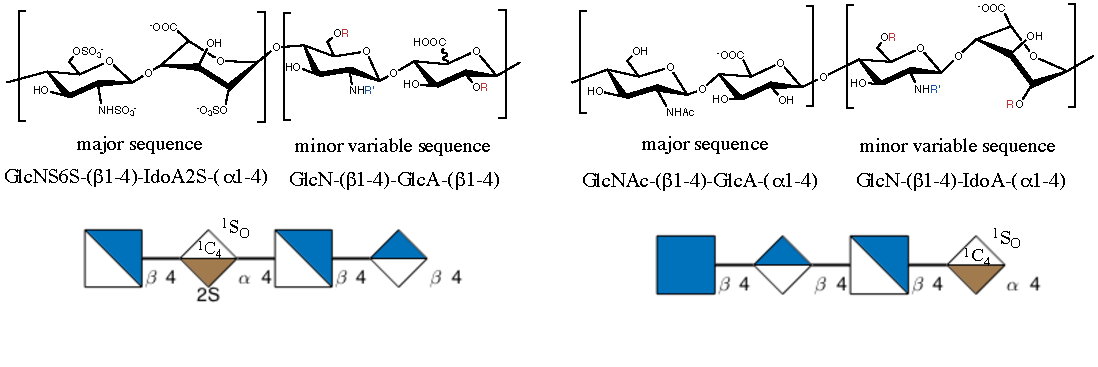
\includegraphics[width=17cm]{HeparinHeparanSulfate.pdf}}
    
    \begin{tabular}{p{1.9cm}|p{0.4\textwidth}p{0.1mm}p{0.36\textwidth}}
   
    
      Location:  & \makecell{\hspace{-1.8cm}\textbullet~  Intracellular compent of \\ \hspace{-1cm} mast cells, esp. lungs, skin.} 
      & &\makecell{\textbullet~ Ubiquitious component of cell \\ \hspace{-1.05cm}surfaces in the ECM.} \\ 
    \renewcommand{\arraystretch}{1}
      Mass: & \textbullet~ 10-12 kDa & & \textbullet~ 10--70 kDa \\
      \renewcommand{\arraystretch}{1.3}
      DoS:  &  \textbullet~ 1.8--2.4 & &  \textbullet~ 0.8--1.8 \\
      GlcA:IdoA & \textbullet~ 1:9 & & \textbullet~ 8:2
    \end{tabular}}
    \caption{The differences between heparin/heparan sulfate, including the chemical structure (R = SO$_{3}$ or H, R' = SO$_{3}$ or Ac), the Symbol Nomenclature for Glycans (SNFG) representation, biological origin, mass, degree of solvation (DoS) and ratios between glucuronic acid to glucosamine residues.}
    
    %\cite{Varki2009SymbolRepresentation} 
    
    \label{fig:HepHS}
\end{figure}

On the surface of all eukariotic cells, highly-sulfated complex polysaccharides known as \acp{GAG} act as emissaries for the reception and modulation of a wide range of proteins, affecting normal physiological processes, such as blood coagulation and neuronal development, as well as serious pathophysiological disorders, such as cancer and Alzhiemer's disease. 
\Ac{Hep} and the closely related \ac{HS} are members of the \ac{GAG} family. \Ac{Hep} possesses the highest negative charge density in all of nature. \ac{Hep} and \ac{HS} bind to \ac{GAG} specific receptors on proteins such as chemokines, cytokines, growth factors, morphogens, enzymes and adhesion molecules\cite{Murphy2007StructuralHeparin, Iozzo2001HeparanArena, Kreuger2006InteractionsSpecificity, Kowitsch2018MedicalReview}. 
In the clinic, \ac{Hep} is a widely used anticoagulant drug to treat patients with thrombic disorders.\cite{Liu2014ChemoenzymaticHeparin.}
Like all \acp{GAG}, these oligosaccharides are comprised of repeating uronic acid residues (\ac{Ido} or its C5 epimer, \ac{GlcA}, which are \textalpha~or  \textbeta 1\textrightarrow4-linked, respectively) paired with \textalpha 1\textrightarrow4-linked \ac{GlcN} residues (Figure \ref{fig:HepHS}). 
Each \ac{GAG} can exhibit various sulfation patterns and \ac{DoS} (the number of sulfo groups per disaccharide), which is a product of around 26 proteins involved in \ac{GAG} biosynthesis in the golgi apparatus.\cite{SoaresdaCosta2017SulfationDisorders, Varki2009BiologicalGlycans}
\ac{HS} occurs in many cell types, however; heparin is isolated exclusively from mast cells.\cite{Liu2014ChemoenzymaticHeparin., Gandhi2008TheProteins}
Here, both sugars are found on the surface of \acp{PG}, where they are can facilliate recognition and cell signalling. 
While \ac{Hep} and \ac{HS} are comprised of similar disaccharide building blocks, their \ac{DoS} and ratios between \ac{GlcA} and \ac{Ido} difers.
\ac{Hep} has higher sulfation levels than HS (\ac{DoS} 2.6 vs 0.6, respectively). 
Upregulation of \ac{Ido} also varies; around 9 in 10 of the disaccharide units in \ac{Hep} contain \ac{Ido}, while only 2 in 10 \ac{HS} disaccharide units contain \ac{Ido}. The structural encoding ability of \acp{GAG} rivals that of DNA, RNA and proteins.\cite{Gama2006SulfationActivity} 
The amino sugar can be sulphated at C4, C6, the unsubstituted nitrogen or C3 (rare), and the uronic acid residue can be substituted at C2 or C3 -- leading to \textgreater1,000,000 possible substitution patterns for a \ac{GAG} octasaccharide.\cite{Gandhi2008TheProteins, SoaresdaCosta2017SulfationDisorders,Gama2006SulfationActivity} 

\begin{figure}[tl!]
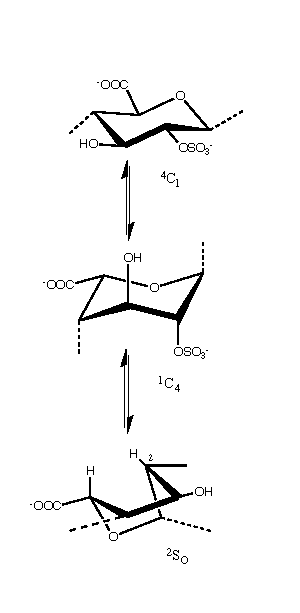
\includegraphics[width=12cm]{ido_confs.pdf}
\caption{\textbf{(A)} Conformational equilibrium of iduronic acid in solution and bound to the protein. \textbf{(B)} The diversity of iduronic ring conformations }
\label{fig:ido_confs}
\end{figure}

Flexible ring conformations of \ac{GAG} components add further structural complexity to the oligosaccharide and are reasoned to have bioloigical relevance during \ac{GAG}--protein interactions.\cite{Sattelle2013DoesHeparanome} 
Although \ac{GlcA} and \ac{GlcN} remain in the standard $^{4}C_{1}$ conformation, the exceptional plasticity of \ac{Ido} ring conformations is unique amongst sugars, and is dependent on its position in the chain, ionic conditions and sulfation pattern.\cite{Capila2002Heparin-proteinInteractions., vanBoeckel1987ConformationalAcid}
At the reducing end, \ac{Ido} has been characterized as existing in an equilibrium between $^{4}C_{1}$, $^{1}C_{4}$ and $^{2}S_{O}$, using $^{1}$H NMR spectroscopy (Figure \ref{fig:ido_confs}).\cite{Ferro1986EvidenceStudies, vanBoeckel1987ConformationalAcid} 
When \ac{Ido} is inside the chain, the equilibrium favors the $^{1}C_{4}$ and $^{2}S_{O}$ conformations exclusively, due to interactions with the 1\textrightarrow4-linked neighbouring sugar.\cite{vanBoeckel1987ConformationalAcid} 
When \ac{Ido} is sulfated at the C2 position, the $^{2}S_{O}$ conformer may become more prominent to minimize unfavorable 1,3 diaxial interactions in the $^{1}C_{4}$ structure.\cite{Hsieh2016UncoveringSulphateb} However, the barrier for interconversion between the two conformers is low and has little effect on the overall conformation of the oligosaccharide, allowing \ac{Ido} to adopt poses suited for specific interactions between basic residues. \cite{Capila2002Heparin-proteinInteractions.} In the case of the \ac{Hep} and \ac{FGF2} complex, two \ac{Ido} residues are poised in $^{1}C_{4}$ and $^{2}S_{O}$ conformations respectively (\ac{PDB} entry 1I8Q),).\cite{Faham1996HeparinFactor} 
Ring flipping, which is believed to occur on the \textmu s timescale based on \ac{MD} simulations, has been a proposed as mechanism for selective binding/unbinding.\cite{Sattelle2012DependenceIdopyranosides} 

{\renewcommand{\arraystretch}{1.5}
\setlength{\tabcolsep}{0.3cm}

\begin{table}[bl!]
    \hspace{}
    \begin{tabular}{p{2cm}p{5.5cm}p{7.5cm}}
        \hline
        Technique & Characterization & Disadvantages  \\
        \hline 
        \makecell[tl]{X-ray \\ crystall--\\ography} & 3D structure of ligand--protein complex in a single low energy conformation & \makecell[tl]{\textbullet $ $ Often errors in residue structures/names\\ \textbullet $ $  Only identifies one conformation\\ \textbullet $ $  Poor resolution can lead to incorrect \\~~~structures\\ \textbullet $ $  Protons are not characterized } \\
        
        NMR & Time averaged angles, dihedrals and distance between protons, structural connectivity & 
        \makecell[tl]{\textbullet $ $ Time averaged structure cannot inform \\ \hspace{3mm} structural ensembles\\ \textbullet $ $  Innappropriate for long (\textgreater\textmu s) timescales \\ \textbullet $ $  Small error in coupling constants result \\ \hspace{3mm} in large structural uncertainty }\\ 
    
        \makecell[tl]{Molecular \\ dynamics} & Simulations of the structure of ligand--protein complexes over time & \makecell[tl]{\textbullet $ $ Relies on accurate forcefields and models \\ \textbullet $ $  Computationally expensive for long \\ \hspace{3mm} (\textgreater\textmu s) timescales}  \\
        \hline
        
    \end{tabular}
    \caption{Experimental and \textit{in silico} methods for characterisation of the 3D structure of glycosaminoglycans.}
    \label{tab:GAGprotein}
\end{table}
}
\begin{figure}[bl!]
    \centering
    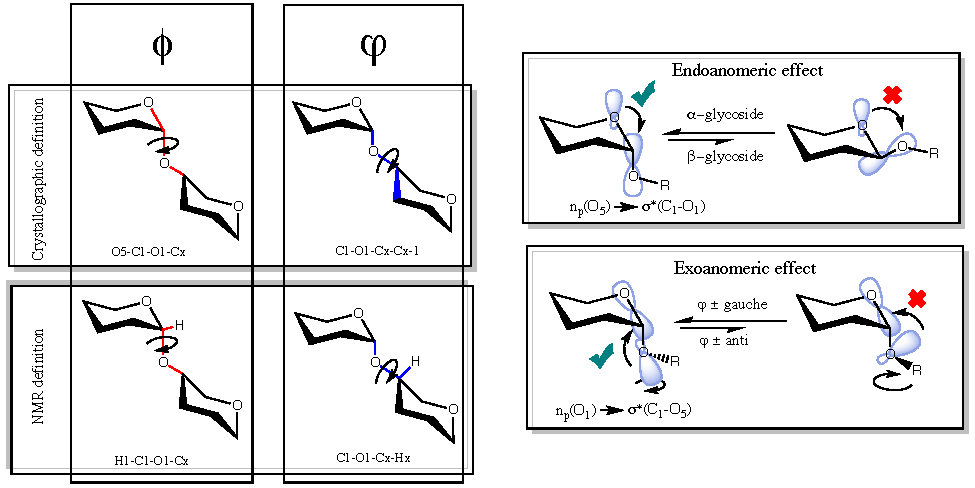
\includegraphics[width=14cm]{phi_psi_endo_exo.pdf}
    \caption{\textbf{(A)} The crystallographic and NMR definitions of the \textphi~ and \textpsi~ torsions of oligosaccharides. \textbf{(B)} The endoanomeric effect as an explanation for the increased stability of \textalpha~--glycosides. \textbf{(C)} The exoanomeric effect as an explanation for the preference of gauche conformations of \textpsi~ torsions. }
    \label{fig:phipsiendoexo}
\end{figure}

Standard NMR techniques struggle dramatically to discriminate between the exchange of even the most simple conformers on the \textmu s timescale - at best only 10\% of conformers are perceptible.\cite{Sattelle2011IsChair} Therefore \ac{MD} simulations are crucial to gain insite into these types of structural equilibria.\cite{Woods2018PredictingComplexes} 
For instance, \ac{GlcNAc} was previously assumed to adopt a stable, $^{4}C_{1}$ chair conformation.\cite{Sattelle2011IsChair} 
However, when crystal structures of ligands conatining GlcNAc residues were obtained, conformer deviations to $^{2}S_{O}$ were observed which suggest that the local chemical environment plays an important role in the 3D structure of the sugar. 
\ac{MD} simulations of GlcNAc in solution, over a 20 \textmu s timescale, reached a conformational equilibrium between 3 - 5 \textmu~ where $^{1}C_{4}$ was the predominant conformer (approx. 99.6\%) and the $^{2}S_{O}$ and other minor conformers were also observed.



\begin{figure}[tl!]
    \centering
    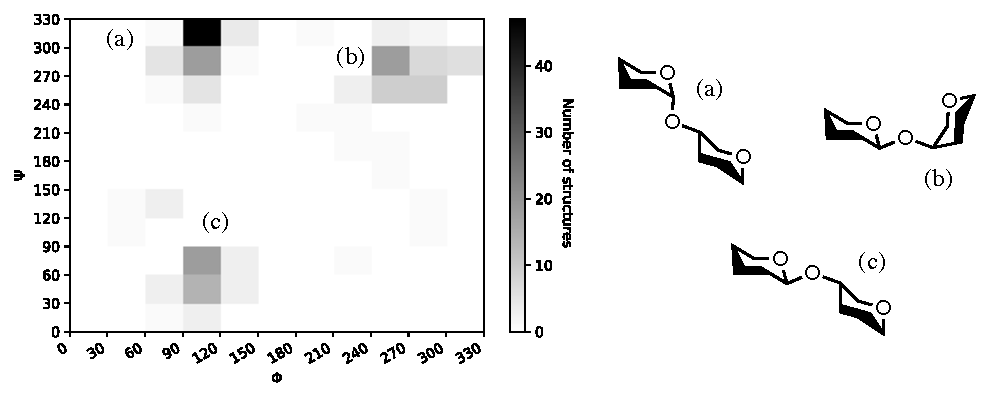
\includegraphics[width=14cm]{phi_psi_distributions.pdf}
    \caption{The distribution of \textphi~and \textpsi~angles of \acp{GAG} structures from the \acf{PDB}.}
    \label{fig:phi_psi_dist}
\end{figure}

Oligosaccharides have two axis of free rotation, or torsions, around the glycosidic linkage, defined as \textphi~and \textphi~(Figure \ref{fig:phipsiendoexo} A). When analysing data from crystallography, the dihedrals, \textphi~and \textphi, may be defined using the atoms O5--C1--O1--CX and C1--O1--C$x$--C$(x-1)$, respectively.
Alternatively, \textphi~and \textphi~may be found using NMR observables (where the dihedrals are defined as H1--C1--O1--C$x$ and C1--O1--C$x$--H$x$, respectively). 
In general, the answer to ``how flexible are the glycosidic linkages inside an oligosaccharides?'' may differ depending on the chemist answering the question. To a protein crystollographer, the absence of secondary or teriary structural elements may prompt them to classify these polymers as flexible. However, a carbohydrate chemist familiar with NMR or crystallographic data, may disagree, since these dihedrals usually only deviate by at most 90\textdegree, when comparing disaccharide pairs that share simillar linkage geometries (i.e. \textalpha~and \textbeta~linkages to axial/equitorial substituents (Figure \ref{fig:phi_psi_dist})). This has been attributed to the exoanomeric effect (Figure \ref{fig:phipsiendoexo} C), where favorable orbital interactions between the non-bonding p-orbital of the oxygen participating in the glycosidic bond and the $\sigma^{*}$ orbital of the O5--C1 bond. This interaction is analogous to the endoanomomeric effect (Figure \ref{fig:phipsiendoexo} B), where favorable orbital interactions between the non-bonding p-orbital of the ring oxygen and the $\sigma^{*}$ orbital of the C1--O1 bond.






% PHI and PSI

% Although the overall helical structure is maintained in the
% FGF-bound HSGAG compared with unbound HSGAG, we observe
% distinct changes in the backbone torsion angles of the oligosaccharide
% chain induced upon protein binding. These changes result in local
% deviations in the helical axis that provide optimal ionic and van der
% Waals contact with the protein. A specific conformation and topological
% arrangement of the HSGAG-binding loops of FGF, on the other
% hand, impose structural constraints that induce the local deviations in
% the HSGAG structure, thereby enabling maximum contact between
% HSGAG and the protein.


\subsubsection{Protein interactions}

\ac{Hep} and \ac{HS} bind to the surface on proteins, due to their size and hydrophillic nature. At physiological pH, all carboxylic acid and sulphate groups are deprotonated. 
These negatively charged moieties recognize shallow pocket regions of positive charge on the protein surface. Residues associated with these positively charged GAG binding surfaces are predominantly Arg and Lys, but His is also involved in some complexes. Of these two main residues, Arg has been shown to bind with 2.5 times more affinity than Lys. The guanidino group in arginine displays stronger electrostatic interactions with sulphate groups, as well as more stable hydrogen boding \cite{Hileman1998Glycosaminoglycan-proteinProteins}. Electrostatic interactions operate over longer distance than those that rely on hydrogen bond or van der Waals forces. Coulombic forces have a $ r^{-1}$  relationship (where $r$ is the distance between two ions), whereas vander Waals forces have a  $ r^{-3}$ to  $ r^{-6}$ dependence. \cite{Sankaranarayanan2014TowardProteins} 
Generally, hydrogen bond distances are between 2 - 4 \AA, whereas the cutoff for charged interactions can be as high as 8 \AA. \cite{FerreiradeFreitas2017APDB}
\acp{GAG} share features in common with DNA; both are linear polymers with a high propensity of negative charge. 
Due the high repulsive energy associated with multiple negatively charged groups, cations (such as Na$^{+}$) bind to minimize these unfavourable forces (although this process is entropically unfavourable)  \cite{Hileman1998Glycosaminoglycan-proteinProteins}
To bind to a protein, a cations coordinated to the \ac{GAG} must be displaced. Simillarly, any anions coordinated to Lys, Arg or His must also be displaced. This is also known as the ``polyelectrolyte effect'' and can be considered a screening effect, since the competing interaction (i.e. GAG--protein binding) must be strong enough to displace these ions.  
As expected, an increase in the concentration of salt reduces ligand binding; \cite{Capila2002Heparin-proteinInteractions., Gandhi2008TheProteins} 
in the case of DNA and heparin, this has been shown by sodium--23 NMR and titrating calorimetry, respectively\cite{Anderson1978Sodium-23Interactions., Thompson1994EnergeticDomain}.  
While charged interactions have been highlighted as important for recognition of the binding site\cite{Samsonov2016ComputationalComplexes}, these interactions are nonspecific: almost any protein surface containing positive charge will recognize a sulfated GAG chain. 

\begin{figure}[bl!]
    \centering
    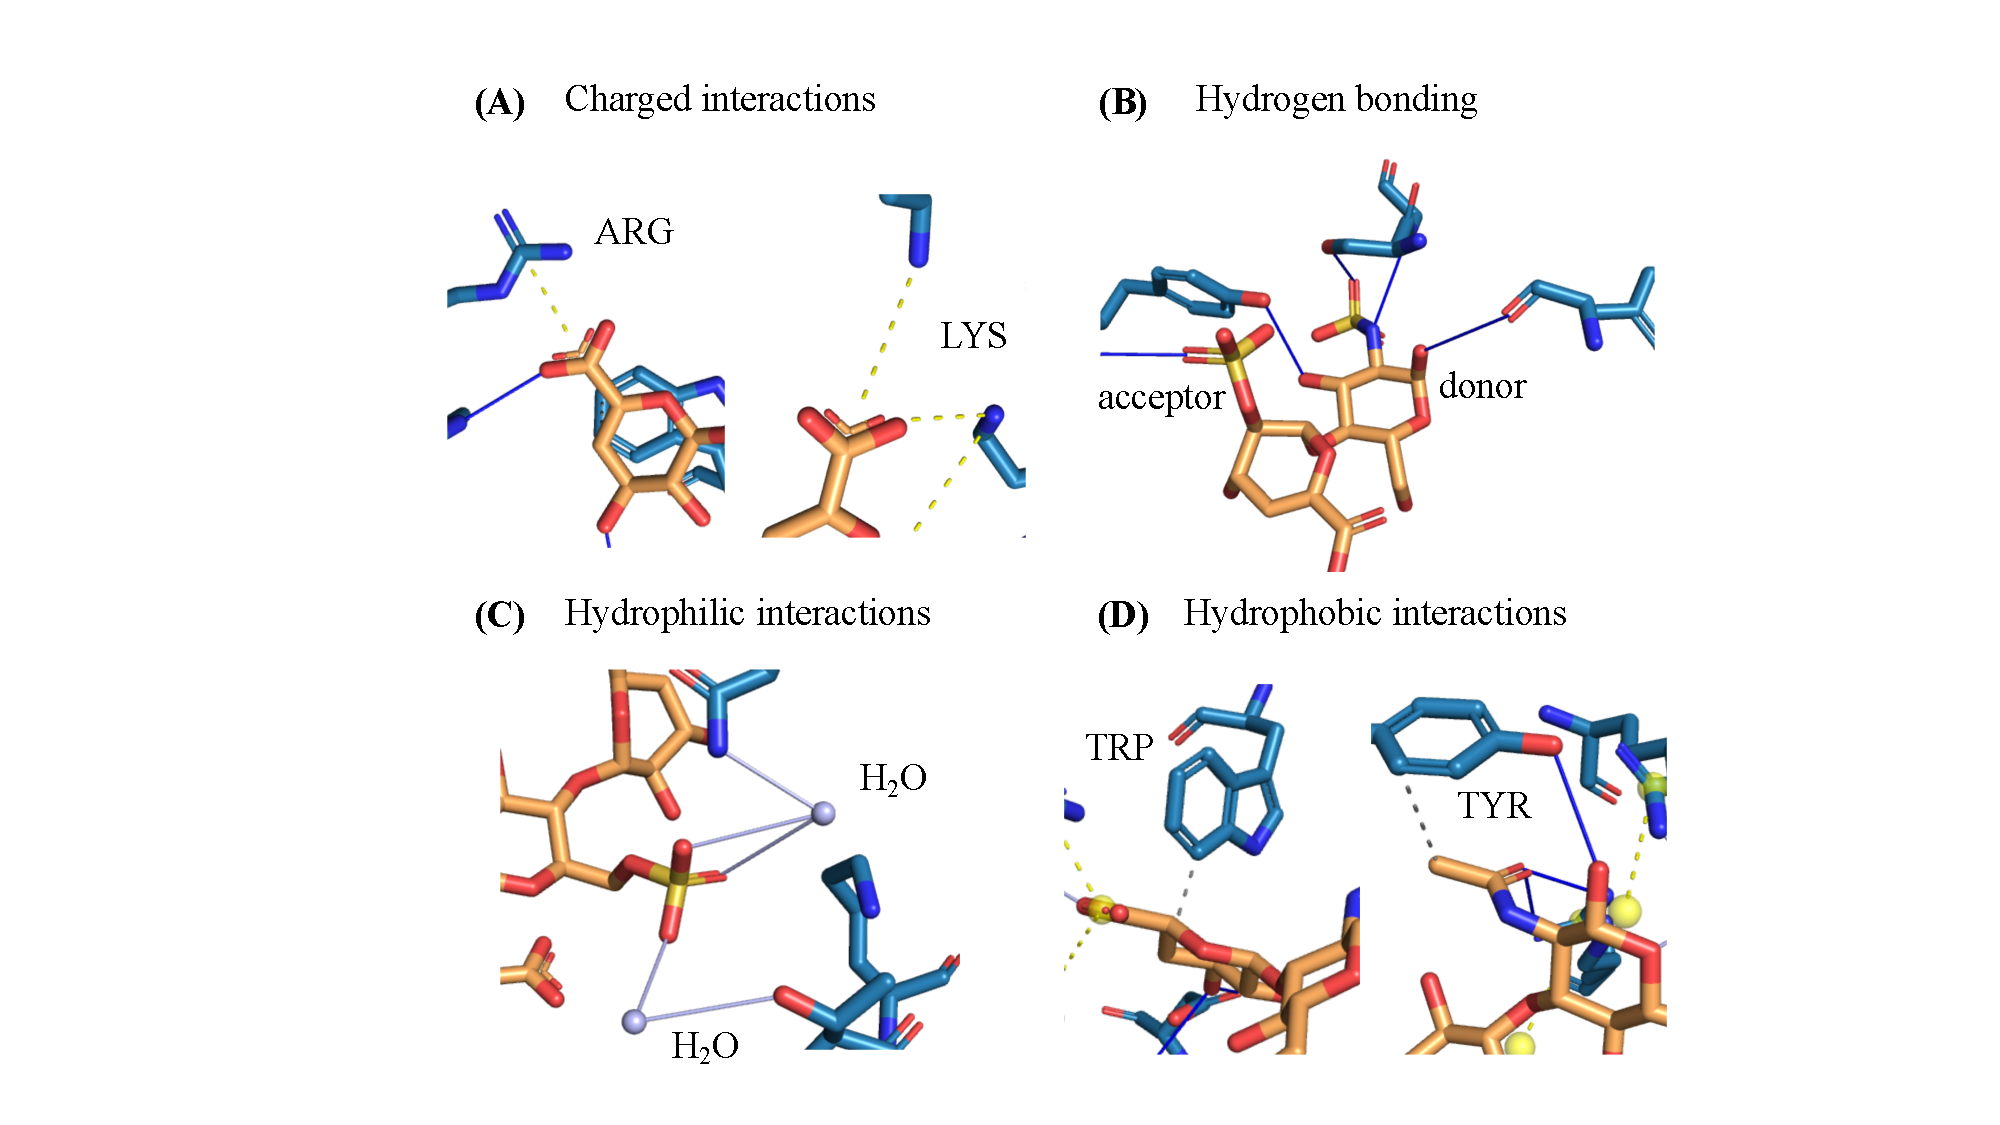
\includegraphics[width=11cm]{interactions.pdf}
    \caption{Examples of four types of non-covalent interactions between GAG--protein complexes, taken from the PDB. \textbf{(A)} Charged interactions, an important non specific interaction, are usually found between carboxylate/sulfonate groups and ARG, LYS or HIS (rare). \textbf{(B)} Hydrogen bonds are a common interaction, due to the large number of hydrogen bond donors/acceptors found in GAGs. \textbf{(C)} Due to their charge, GAGs are often solvated by water residues. \textbf{(D)} Hydrophobic residues, usually TRP or TYP, usually interact with GAGs \textit{via} C--H - - - \textpi~interactions.}
    \label{fig:interactions}
\end{figure}


It is hydrogen bonding that is the prevailing interaction to determine the specificity of \ac{GAG}--protein interactions. In general, carbohydrates form hydrogen bonds with side chain residues of polar planar amino acid residues. \cite{Malik2007SequenceNetwork}
These hydrogen bonds can be cooperative hydrogen bonds, bidentate hydrogen bonds or hydrogen bond networks and facilitate low energy conformations of the polysaccharide.\cite{Quiocho1989Protein-carbohydrateFeatures}  
The free energy for hydrogen bonding can vary between −0.5 kcal mol$^{-1}$ (for neutral hydrogen bonds) to −4.7 kcal mol$^{-1}$ (for charged hydrogen bonds) \cite{Davis1997HydrogenHypothesis}. However, the contribution of a hydrogen bond to binding can be very modest (or penalizing) if the new interaction formed does not outweigh the desolvation penalty upon ligand binding. \cite{H.Williams1998AspectsInteractions}

The thermodynamic consequences associated with desolvation of these highly charged oligosaccharides is trade-off that has an immense effect on the binding affinity of the ligand.\cite{Gandhi2009FreeInteractions, Samsonov2014FlexibilitySystems}
The desolvation penalty is large and positive and scales with increasing size and charge of the sugar.\cite{Gandhi2009FreeInteractions, Samsonov2014FlexibilitySystems} 
Only ligand poses with favourable orientations of charged and hydrogen bond acceptor moieties are capable of off-setting this penalty and binding strongly with the protein. \cite{Bryce2001Carbohydrate-ProteinA}
For this reason, \ac{GAG} crystal structures are generally observed with a shell of water molecules partially covering portions of the ligand. \cite{Gandhi2009FreeInteractions, Capila2002Heparin-proteinInteractions.}

Statistical analyses of general carbohydrate-binding protein sequences indicate that, for amino acids with hydrophobic side chains, Trp is the most highly represented when considering the amino acids participating carbohydrate-binding. \cite{Malik2007SequenceNetwork, Shionyu-Mitsuyama2003AnProteins}. 
The aromatic residue Trp has a significantly higher mean solvent accessibility in carbohydrate binding locations, whereas aliphatic residues (Ala, Gly, Ile and Leu) are more hydrophobic and not commonly found on the surface of proteins where sugar binding occurs. \cite{Malik2007SequenceNetwork, Shionyu-Mitsuyama2003AnProteins}. 
The aromatic ring in Trp can pack against the hydrophobic face of a sugar molecule, perpendicular to the C--H of the sugar. \cite{Gandhi2008TheProteins} 
This can be seen in the \ac{PDB} (PDB entry 1I8Q), where 4-deoxy-\small{D}-glucuronic acid is orientated at 90\textdegree~from the Trp, an orientation which allows for simultaneous hydrogen bonding to an Asp residue and charge-charge interactions with an Arg residue.\cite{Li2001HyaluronanLyase.}
Tyr, which is a hydrophobic aromatic residue which is perhaps more frequent in GAG--protein complexes due to the aromatic alcohol being a possible hydrogen bond donor, has been shown to allow for concurrent hydrogen bonding and C--H - - - \textpi~interactions, specifically with GlcNAc at favourable orientations (usually the faces of the sugar and the aromatic ring are 90\textdegree~apart), this can be observed in an example taken from the \ac{PDB} (PDB entry 1HM3). 
\cite{WeijunHuang2001ActiveMutagenesis}
Overall, the free energy of interaction, which is related to the observed dissociation constant (K$_{d}$), has contributions from the polyelectrolyte effect, hydrogen bonding, and hydrophobic interactions. \cite{Thompson1994EnergeticDomain}

Structural similaries in 21 heparin-binding proteins, observed by Cardin and Weintraub, propose a consensus sequence of XBBXBX or XBBBXXBX, where B is a lysine or arginine (with a very rare occurrence of His) and X is a hydropathic residue, for heparin-binding proteins. When these Cardin--Weintraub sequences form \textalpha-helices, it is not uncommon for the spacing of these basic residues to allow for interactions on one face of the helix. \cite{Capila2002Heparin-proteinInteractions.} 
Cardin and Weintraub sequences offer limited predictive value for heparin binding sites, as \acp{GAG}, in general, do not interact solely with one chain of the protein.\cite{Capila2002Heparin-proteinInteractions., Gandhi2008TheProteins} 
Due to this, a 3D analysis of the binding site similarities is required.

\subsubsection{Deciphering the so-called `sulfation code'}

\begin{figure}[bl!]
    \centering
    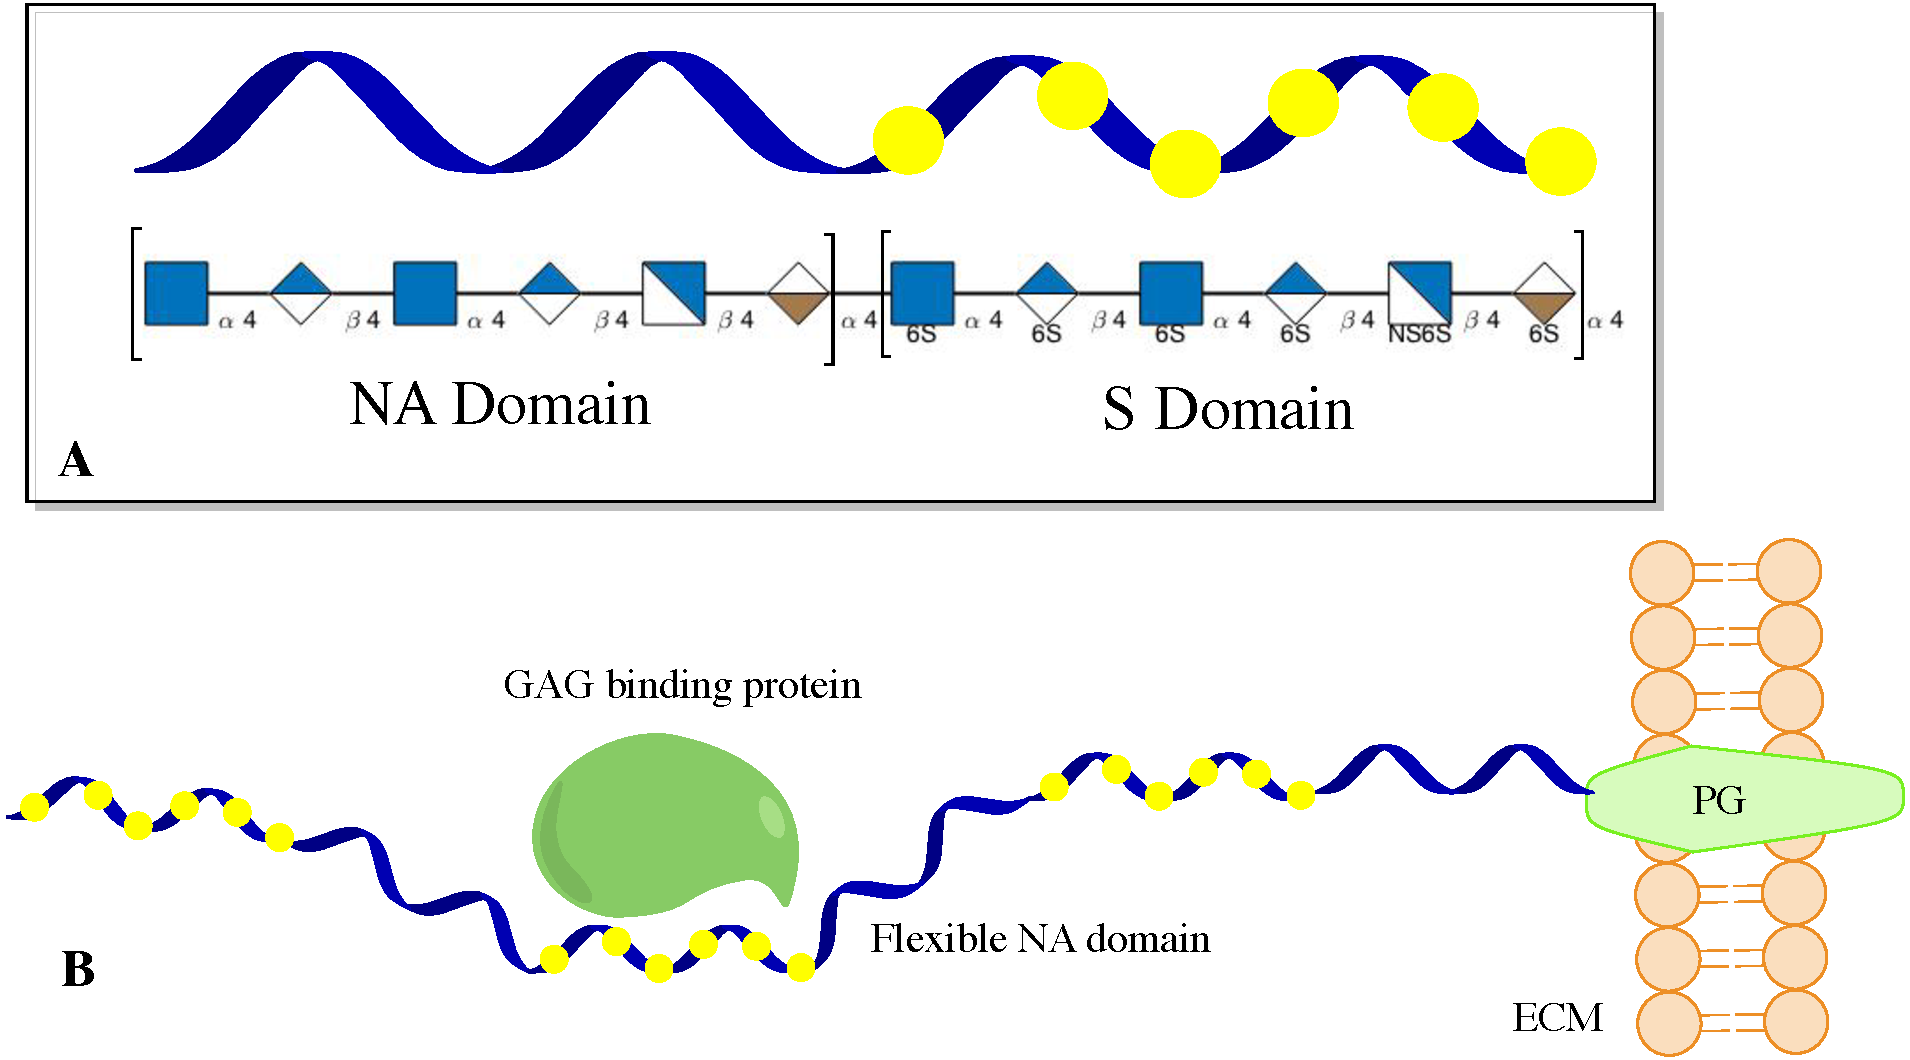
\includegraphics[width=13cm]{NAandSdomain.pdf}
    \caption{\textbf{(A)} Example of the GAG sequences (depicted in SNFG notation) showing the non-sulfated region (NA domain) and the sulfated region (S domain). \textbf{(B)} A cartoon representation of the induced fit between GAGs and proteins, faciliated by the flexable, non-sulfated domain.}
    \label{fig:Sdomain}
\end{figure}

\ac{GAG} sulfation patterns have been the subject of multiple \ac{SAR} studies, which have suggested high specificity in relation to function in some cases.\cite{Habuchi2004SulfationCode, Gama2006SulfationActivity} 
In contrast, some \ac{GAG}--protein interactions have been shown to be entirely general (i.e. MIP-1\textalpha~can be inhibited by sulfated oligosaccharides regardless of \ac{GAG} family. \cite{Kuschert1999GlycosaminoglycansResponses}
For this reason, GAG sulfation patterns have been likened to the “sulfation code”. \cite{Habuchi2004SulfationCode, Swarup2013SugarNeurons, Kowitsch2018MedicalReview, Gama2006SulfationActivity}
It is not only the specific sequences of sugars that effects GAG--protein interactions, but the sugars location in chain which also plays a role in this complex phenomenon. 
`Neighbourhoods' of varying sulfation levels in the oligosaccharide determine S and N domains (sequences with high and low levels of sulfation respectively) (Figure \ref{fig:Sdomain} (A)). 
The conformation of IdoA is regulated by the sulphation pattern of itself and nearby saccharides. \cite{Hsieh2016UncoveringSulphate}.
The 2-O sulfate groups of iduronic acid and 6-O and N sulfate groups on neighbouring hexosamine residues, can strongly favour the $^{1}C_{4}$ Ido conformation, which causes a kink to the chain. \cite{Raman2005StructuralInteractions}
The NA domain has also been shown to introduce more flexibility to the chain and can allow the polymer to bridge across multiple binding sites of a protein (Figure \ref{fig:Sdomain} (B)). \cite{Capila2002Heparin-proteinInteractions., Nahain2018HeparinActivity, Li2004StructureHeparin, Dementiev2004TheSpecificity}

\begin{figure}[tl!]
    \centering
    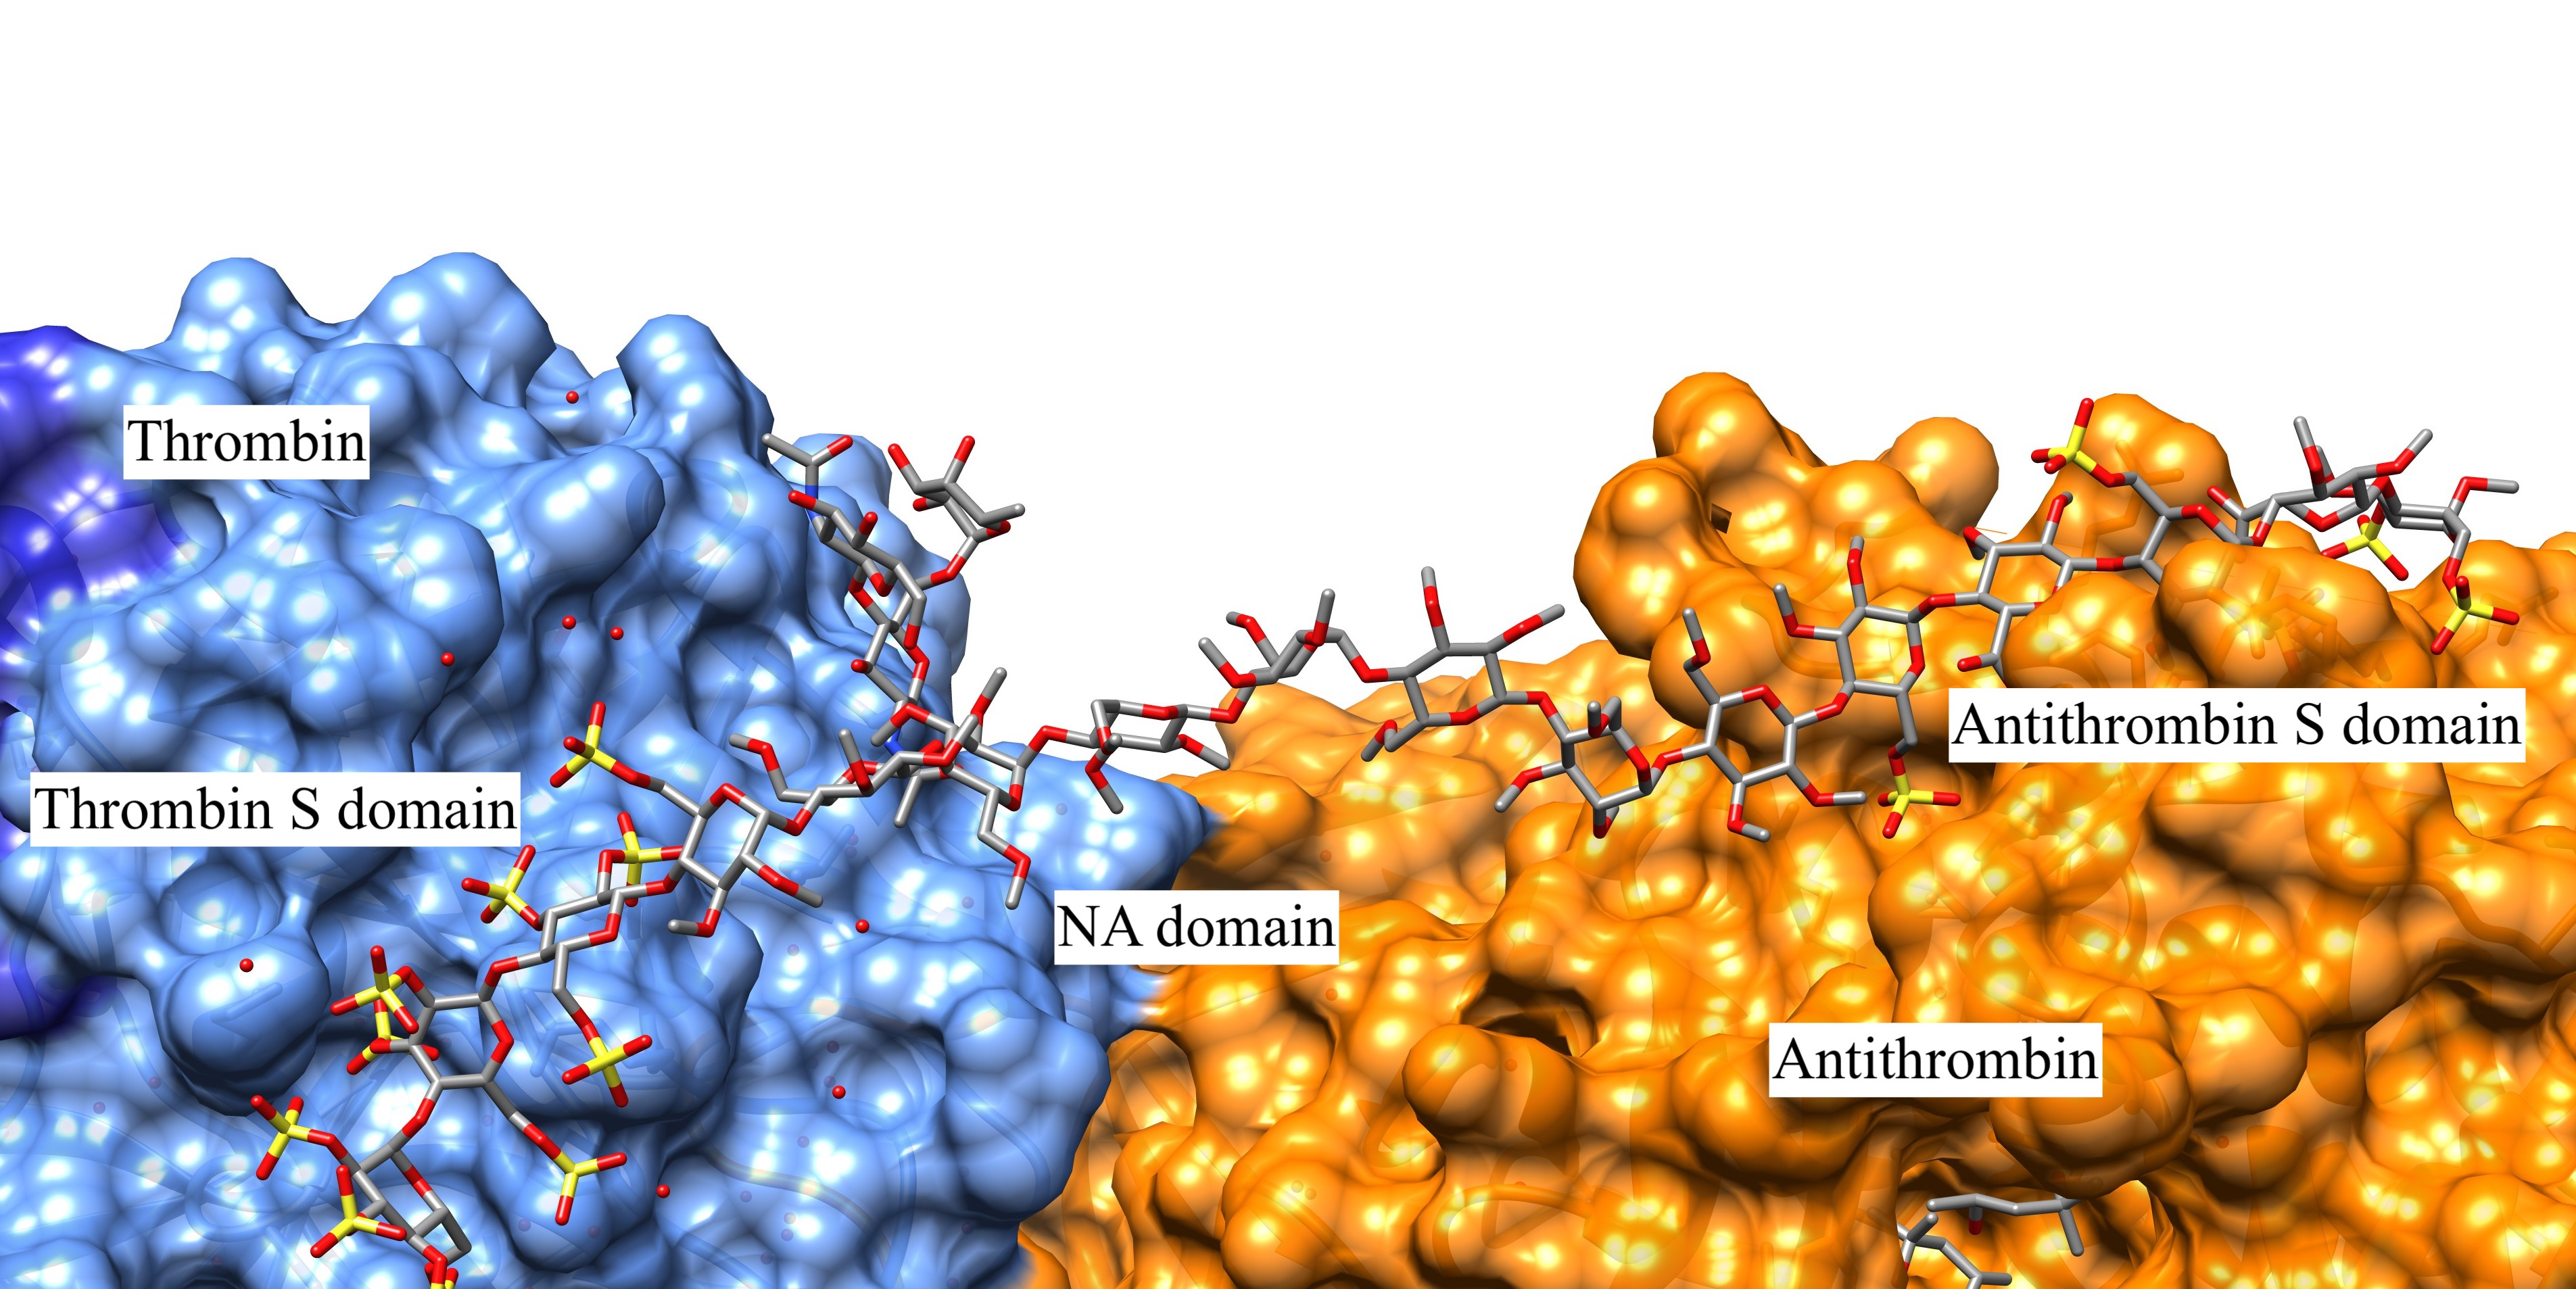
\includegraphics[width=13cm]{AntiThrombinThrombinHeparinMimetic.jpg}
    \caption{The ternary complex of antithrombin, thrombin and a 16-mer synthetic heparin mimetic, coloured by chain, showcasing the complimentary roles of S and NA domains during GAG binding, which can allow for recognition and flexibility, respectively (PDB entry 1TB6).}
    \label{fig:ternary}
\end{figure}

The prototypical example of this is the mechanism of thrombin inhibition which drives the efficacy of heparin as an anticoagulant. \cite{Li2004StructureHeparin, Dementiev2004TheSpecificity}
Antithrombin, the principal physiological inhibitor of thrombin, requires the formation of a ternary complex (antithrombin--heparin--thrombin) for inhibition to occur.\cite{Capila2002Heparin-proteinInteractions., Nahain2018HeparinActivity} In this complex, antithrombin, a serpin protein, recognizes a highly specific heparin pentasaccharide sequence through initial weak electrostatic interactions which causes a conformational change. If the heparin polymer is long enough (and flexible enough), it can bind non-specifically to thrombin on the opposite side of the chain. The thrombin protein can direct itself towards antithrombin in the correct orientation, effectively using the oligosaccharide chain as a guide rope.\cite{Li2004StructureHeparin, Dementiev2004TheSpecificity} This assistance provided by oligosaccharide increases the antithrombin induced inhibition of thrombin by 4000 fold. \cite{Li2004StructureHeparin, Dementiev2004TheSpecificity} 
This ternary complex has been characterized in stunning detail with 16-mer synthetic heparin mimetic using x-ray crystallography (Figure \ref{fig:ternary}, PDB entry 1TB6).\cite{Dementiev2004TheSpecificity}

Due to the immense variation in \ac{GAG} oligosaccharides, isolating defined sulfation sequences from biological sources is understandably difficult and is often a task left to overcome by the synthetic chemist.  \cite{Gama2006SulfationActivity}
These synthetic procedures are generally non-trivial. \cite{Das2001SynthesisHeparin} 
Futhermore, the methods available for characterization of 
\ac{GAG}--protein interactions at the atomistic level (x-ray crystallography and protein NMR) are by no means poised for use as high-throughput techniques. This pushes the problem of thoroughly rationalizing \ac{GAG}--protein interactions firmly into the hands of computational chemists and necessitates the development of computational techniques for understanding these essential biomolecules. \cite{Woods2018PredictingComplexes}

%
%
% Carbohydrates in computation
%
%
%

\subsection{Carbohydrates in computation}
\subsubsection{Overview}

\begin{figure}[bl!]
    \centering
    \includegraphics{"computational techniques".pdf}
    \caption{An explanation and comparison of three computational techniques: quantum mechanics, molecular dynamics and docking. The limitations of each method, and how each method can be used in conjunction to mitigate said limitations, is highlighted.}
    \label{fig:comp}
\end{figure}

Computational chemistry techniques, which attempt to calculate the free energy of a system, can be separated into two classes based on the smallest measurable unit considered in the calculation: \ac{QM}, where the electron is the smallest particle of interest; and \acf{MD}, where the smallest particle is the atom. \cite{}
For problems such as probing chemically interesting \ac{GAG}--protein interactions, nonempircal methods, such as `docking', can be used.

To quantify the efficiency of these computational techniques, it is convienient to introduce a notion from computer science: time complexity (commonly represented as $\mathcal{O}(f(n))$). Time complexity relates the size of a task, $n$, to the time taken to complete the task, $f(n)$. The units of size and time are arbituary and should be defined by the author. A task of $\mathcal{O}(n^{2})$ implies a quadratic relationship between the size of the task and the time taken to complete it. Examples of time complexity relationships relavent to computational chemistry are given in Figure \ref{fig:timecomplexity}.

\begin{figure}[tl!]
    \centering
    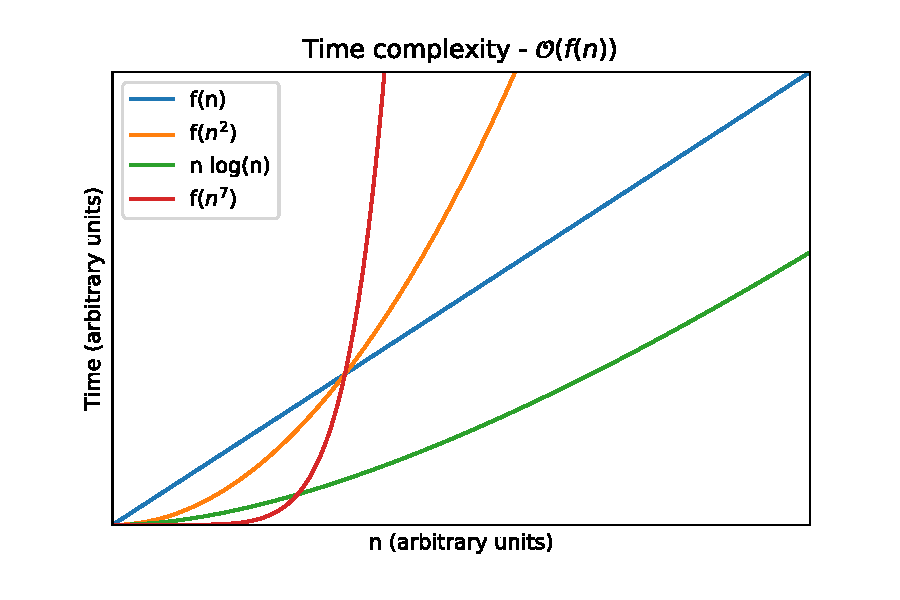
\includegraphics[width=9cm]{timecomplexity.pdf}
    \caption{Visualization of selected time complexity relationships, i.e. $\mathcal{O}(f(n))$, relevant to computational chemistry. For instance, highly accurate quantum mechanics calculations scale $\mathcal{O}(n^{7})$ (n is the number of model electronic orbitals), while simple energy scoring functions in docking programs can be as efficient as $\mathcal{O}(n^{2})$ (n being the number of atoms).}
    \label{fig:timecomplexity}
\end{figure}

\subsubsection{Quantum mechanics}
\Ac{QM} is ...
\Ac{QM} has the ability to give reliable results, such as energies and geometries, that can be used to give approximations using `cheaper' computational methods (such as force fields or energy functions for docking experiments). 

GLYCAM06, an Amber forcefield that provides the basis of energy calculations in VinaCarb, was parameterized using the HF/6-31G* level of theory for geometry optimization and B3LYP/6-3111G(2d,2p) for single point energy calculations\cite{Kirschner2008GLYCAM06:Carbohydrates}. 
During geometry optimization, diffuse functions were added to anionic molecules; however, this approach was not taken during the calculation of single point energies. It is likely therefore, that free energies may be underestimated for anionic compounds. Since solvation effects are key considered key to understanding the thermodynamics of carbohydrates, especially highly charged sugars such as \acp{GAG}, since the parameterization of GLYCAM06 neglected the use of appropriate implicit solvents, such as water, it would be prudent to consider this error when evaluating the accuracy of this model. 

In terms of how this functional/basis set combination performs to higher levels of theory, there has been some effort made to benchmark these details when studying these molecules with \ac{DFT}. Although many examples of its use exist in the literature, B3LYP has shown to perform poorly when compared to high level \textit{ab initio} calculations, such as MP2/aug-cc-pVTZ and CCSD(T). CCSD(T) methods scale $\mathcal{O}(n^{7})$ in terms of system size, making high quality calculations of disaccharides prohibitively expensive with current technology. 

GLYCAM06 shows an unsatisfying performance in the entire energy window

A bench marking study involving 

M06-L performed 

\subsubsection{Molecular dynamics}
\Ac{MD}

\subsubsection{Docking}



The distribution of amino acid residues at carbohydrate binding sites suggests

\subsection{Current advances in GAG/carbohydrate docking}

\subsubsection{Cluspro: heparin site mapping (2014)}

The Cluspro server is an online protein--protein docking package which was adapted in 2014 to include a tool used for \ac{Hep}/\ac{HS} site mapping tool.\cite{Comeau2007ClusPro:Server, Mottarella2014DockingProteins,Kozakov2017TheDocking.} 
Cluspro performs three main computational procedures: \ac{RBD}, \ac{RMSD} clustering and refinement using an energy minimization function.\cite{Kozakov2017TheDocking.} 


\subsubsection{VinaCarb (AutoDock Vina) (2016)}
\ac{RMSD}
\ac{PRMSD}

\subsubsection{GAG--Dock (DarwinDock/GenDock) (2017)}
The ``GAG-Dock" method reported by
\citeauthor{Griffith2017PredictingGrowth}\cite{Griffith2017PredictingGrowth} was developed using DarwinDock and GenDock to model GAG--protein interactions. This method accurately predicted \ac{Hep} binding poses within 0.70 - 1.51 \r{A} \ac{RMSD} of the crystal structures (\ac{FGF1}, \ac{FGF2}, and \ac{AT3}. The authors also investigated the specificity of protein binding, through in silico mutations, to favor a particular GAG sulfation pattern. 
To establish the available space for a ligand to dock, a modified version of the sphgen program\cite{Moustakas2006Development5} was used. Sphgen generates concentric spheres that combine to form a curve topology which is used to model the surface of the protein. 
Sphgen can also be used to analysing clustering of docked ligands.\cite{Hendrix1998SurfaceDocking.}
To model \ac{GAG} binding to flat surface, the available space for ligands to bing to flat protein surfaces was increased. In this modification, the “dotlim” parameter in sphgen was altered. The default ``dotlim" value, zero, prevents generation of large spheres with close surface contacts.\cite{Hendrix1998SurfaceDocking.} For \acp{GAG} ``dotlim" parameter was decreased to - 0.9, which allowed for spheres to be generated for flat surfaces.\cite{Griffith2017PredictingGrowth} To prevent sampling from pockets inside the protein that would be inaccessible to \asp{GAG}, a two sphere surfaces are generated by using the normal probe radius the normal 1.4 \r{A} and a larger radius of 2.8 \r{A}. The intersection of these surfaces is taken to generate spheres on the protein surface without sampling from too close to, or outside of, the surface.\cite{Griffith2017PredictingGrowth} 

\subsection{Current challenges in glycosaminoglycan docking}

a very important issue for specificity (Canales et al. 2006), bioactivity (Guerrini et al. 2008) and thermodynamics of protein–GAG interaction (Samsonov and Pisabarro 2013) is represented by conformational space of uronic acid derivatives within GAGs. Because its proper sampling is achieved at microsecond timescales (Sattelle et al. 2010, 2015), which are much longer than conventional molecular dynamics (MD) timescales, rigorous treatment of uronic sugar rings is computationally very expensive. \cite{Samsonov2016ComputationalComplexes}

This is due to the fact that (i) positively charged residues participating in GAG binding have long side chains and, therefore, exploring their conformational space is crucial for predicting GAG binding (Möbius et al. 2013); (ii) protein–GAG complexes reveal poor geometric complementarity between the receptor and the ligand in their interfaces (Taroni et al. 2000); (iii) water molecules can play a crucial role for GAG binding and they should be, therefore, taken into account properly (Samsonov et al. 2011); (iv) there is still a lack of specific docking tools containing scoring schemes developed for GAGs. For these reasons, implementation of experimental data-based restraints can be particularly very beneficial for guiding docking approaches (Seyfried et al. 2007; Hofmann et al. 2015).

\pagebreak
\section{Aims}

\section{Methods}



}
\newpage
{\setstretch{0}
\bibliography{ref}
}

%%%% uncomment for appendix

% \newpage

% \section{Appendix}

% \begin{figure}
%     \centering
%     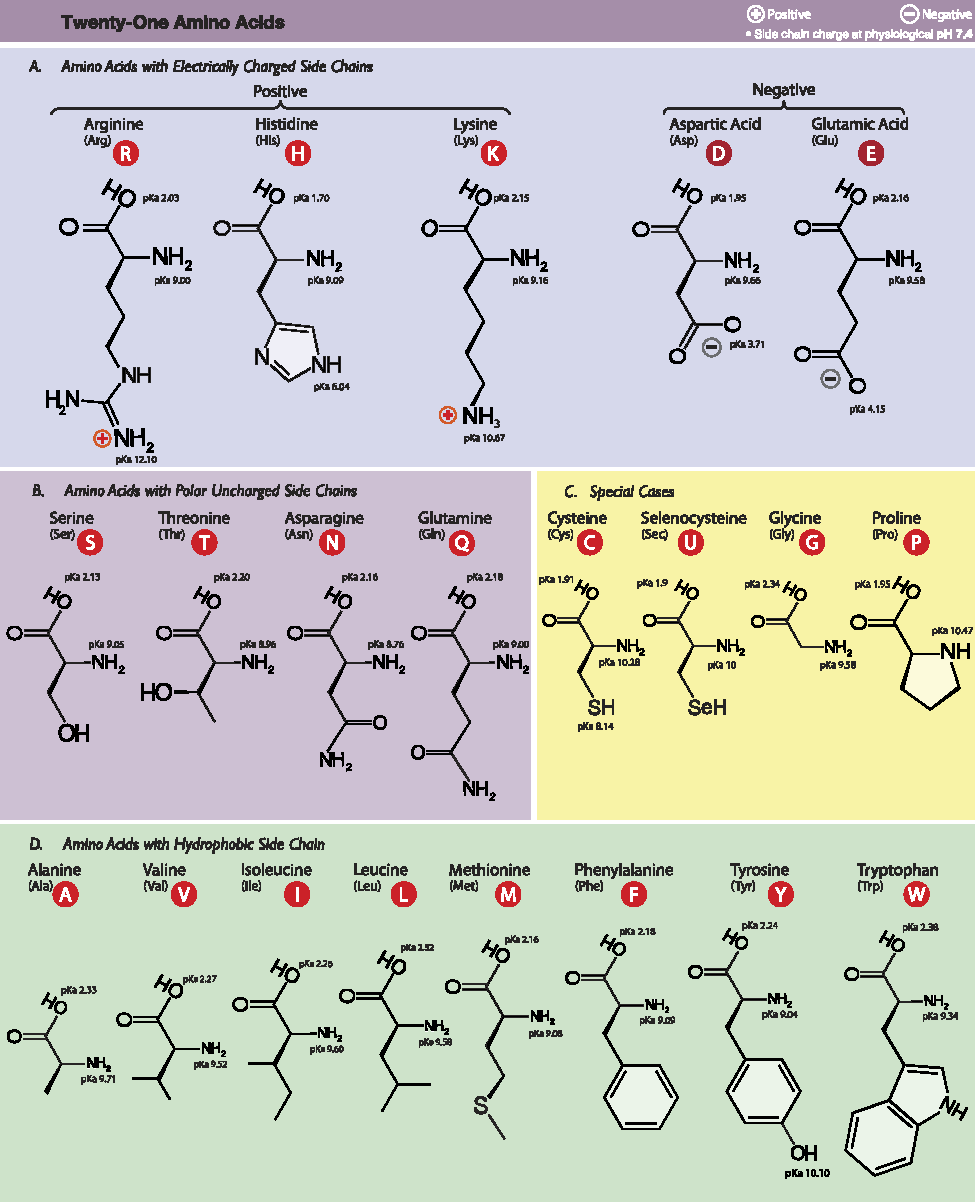
\includegraphics{amino_acids.pdf}
%     \caption{The 21 standard amino acids.}
%     \label{fig:aminoacids}
% \end{figure}

% {\renewcommand{\arraystretch}{1.5}
% \begin{table}[b!]
%     \begin{tabular}{p{5cm}p{6cm}p{3cm}}
%         \hline
%         Heparin--binding protein & Physiological/pathological role & GAG family  \\
%         \hline
%         AT III & Blood coagulation cascade & Hep \\
%         AT III & Blood coagulation cascade & Hep \\
%         AT III & Blood coagulation cascade & Hep \\
%         AT III & Blood coagulation cascade & Hep \\
%         AT III & Blood coagulation cascade & Hep 
%     \end{tabular}
%     \caption{Physiological/pathological effects of Hep/HS--protein interactions.}
%     \label{tab:GAGprotein}
% \end{table}
% }

\end{document}

